\chapter{Prototypical Implementation}
\label{ch:prototype}

\vspace{-1cm}
\begin{center}
Eduard Hirsch
\end{center}

\section{Project Structure}
\label{sec:project-structure}

Before introducing the actual architecture and implementation the structure of the project is described in order to know what to find where. In figure \ref{fig:directory-structure} the main directories are shown which also separate the main components of the business network.

\begin{figure}[htbp]
\centering
\begin{minipage}{5cm}
\dirtree{%
.1 Interlace Blockchain.
	.2 chain.
	.2 fabric.
	.2 webapp.
}
\end{minipage}
\caption{\bf\small Project Directory Structure}
\label{fig:directory-structure}
\end{figure}

Explaining further the folder \textit{"chain"}  contains a \textit{hyperledger composer} implementation of a business network. This business network is the main implementation of the Interlace efforts of creating a working block-chain, which consists mainly of chain-code implementations. But also scripts to deploy and update the chain-code as well as making the network accessible by starting it on the hyperledger fabric chain. 

\textit{"fabric"} is the hyperldger fabric base block-chain needed for running a business network where the chain-code bits are executed on. The chain-code bits from directory \textit{chain} are compiled to a \textit{.bna} file which are then deployed to a fabric network. Those bna-files (also called banana files) can't be used by default by hyperledger fabric. They are rather part of a virtual environment like infrastructure provided by hyperledger composer. Thus the API components of composer provide wrappers to make a composer implementation run on a pure fabric network.

Finally a web application has been implemented which uses AngularJS, a front-end framework provided by Google,  to work with the block-chain. That application is found in \textit{webapp}. This application uses a Swagger\footnote{\url{https://swagger.io/}} based REST-server implementation which comes with hyperledger composer framework.

A more detailed description of the directory structures can be found in subsequent sections where the respective parts are explained in depth.

\section{Architecture}

The core architecture of the INTERLACE project presented next is multi-layered and concentrates on being scalable and highly distributable in contrast to the current monolithic payment platform used by Sardex.

The chosen block-chain approach is going to be explained in detail. The technical challenges during the planning of that implementation strategies are discussed in subsequent sections of that chapter.

\subsection{Sardex Network}

In deliverable D2.1 and D3.1 the current architecture has been written down using the AS(I)M approach and as mentioned before a working client-server application based on message-passing has been developed. This application was realized using the ICEF-framework which is founded on abstract state machines applying a programming language similar to ASM logic definitions.

That classic model was used to derive a new payment network based on block-chain approach. The thoughts for the new network comprise using a publicly maintained and an easy to use block-chain which supports the idea of a interest-free mutual credit system enabling account based balances rather than token based currencies only. These thoughts led to a prototypical implementation using hyperledger fabric together with hyperledger composer.

Regardless of the choice of hyperledger environment it also has been important having a central payment network which is not only reliable and verifiable but also (to a specific extend) controllable in order to impose the basic Sardex payment rules on it.

\subsection{Hyperledger Fabric Network}

The given network constraints were used while creating a new hyperledger fabric network which sets up a core environment offering a basic block-chain to interact with. Next a close look is taken on the actual implemented network and a description for the various parts is given.

In figure \ref{fig:prototype-net} the current working environment is shown. It is utilising the possibilities hyperledger fabric is offering. When looking further into detail fabric actually imposes a structure to a newly created network for which the following main components can be singled out when focusing on Interlace:

\begin{itemize}
	\item Sardex as participating \textbf{organisation}
		\subitem One  \textbf{peer} (named: peer0.sardex.sardex.net)
		\subitem Clients and Services connecting to the network
		\subitem Sardex Membership Provider \textbf{(MSP)} with ID SardexMSP
	\item "Interlace" pseudo organisation
		\subitem An \textbf{orderer} (named: orderer.sardex.net)
		\subitem Interlace Membership Provider \textbf{(MSP)} with ID InterlaceOrdererMSP
	\item Certification Authority short \textbf{CA}
\end{itemize}

Starting from a Certification Authority (\textbf{CA}) a user may issue a unique identity which can be verified any time by anyone participating in the network. Those identities are part of the process of giving members of the circuit right to work with and facilitate the network with particular roles and access privileges. The actual empowering of a user takes place inside of the membership provider (\textbf{MSB}).

Nevertheless, the power of an MSP goes beyond simply caring about who is a network participant or member of a particular channel. An MSP is able of identifying specific roles an actor might play either within the scope of the organization the MSP represents (e.g., admins, or as members of a sub-organization group), and defines the foundation for giving access privileges in the context of a network and channel (e.g., channel admins, readers, writers). More details can be found on the documentations web-site of hyperledger fabric\footnote{\url{https://hyperledger-fabric.readthedocs.io/en/master/membership/membership.html}}.

Due to simplicity reasons and in order to set-up the prototype network quickly, access/role management has been reduced to a minimum. Section \ref{sec:id-management} focus on a more detailed explanation on how those things might work or might be changed to in case of large scale scenarios.  

\begin{figure}[htbp]
  \centering
  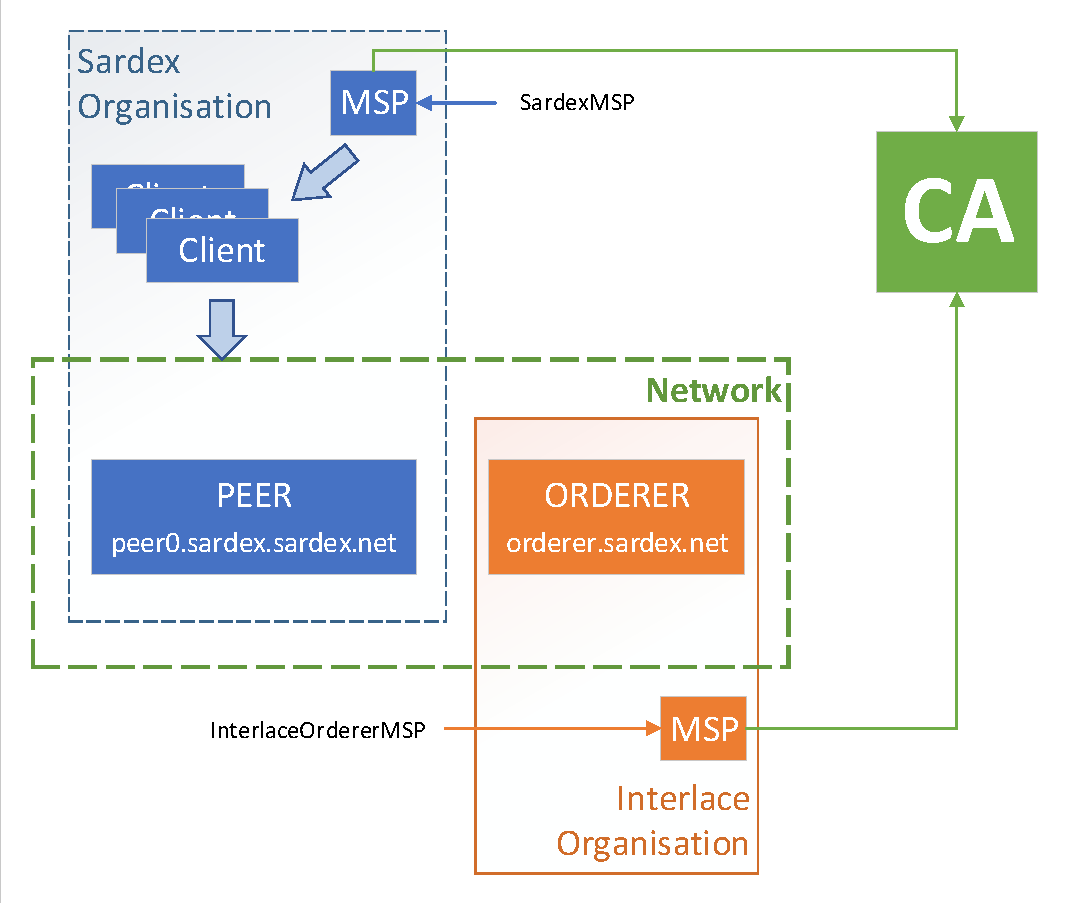
\includegraphics[width=0.5\textwidth, clip, trim=1mm 1mm 1mm 1mm]{Figures/basic-network}
  \caption{\bf\small Network structure implemented by the Prototype}
  \label{fig:prototype-net}
\end{figure}

The single \textbf{orderer} node of figure \ref{fig:prototype-net} takes care to establish atomic broadcasts, orders/batches transactions and also signs each batch (block) to create unique and well defined chains. The membership provider of the orderer uses a central and pre-configured certification authority \textbf{CA}.

For the network one \textbf{peer} is configured and started. This peer can be called the core of the environment because it is mainly handling so called \textit{smart logic} (chain-code) part. Being more specific peers are maintaining the ledger by first endorsing transactions (e.g. credit and debit transfers in case of Interlace), which is done by simulating them, and then they are finally validated and committed to the local ledger.

A very simple network is defined and described by the above scenario, which can be set-up following the instructions of section \ref{sec:prototype}. Certainly, that scenario needs to be extended in a real-world environment, thus a few hints and considerations are given by figure \ref{fig:prototype-net-ext} which will be explained in chapter \ref{ch:conclusion} section \ref{sec:future-scene}.

\subsection{Network Configuration Files}
\label{sec:net-conf-files}

There are three main configuration files providing a basic foundation for generating a preconfigured network. Those files are used to create the respective certificates as well as configuration files to spin up virtualized containers. Thus the following three yaml-files are an example of how to create a particular net as described in the previous section where the Interlace network has been shown:

\begin{enumerate}
	\item crypto-config.yaml
	\item configfx.yaml
	\item docker-compose.yaml
\end{enumerate}

\textbf{crypto-config.yaml}

The \textit{crypto-config.yaml} contains the network topology and defines therefore the basic structure of it. With the configuration file it is possible to use a tool called \textit{cryptogen} which takes crypto-config.yaml as input to generate the cryptographic material necessary to run the block-chain. Being more specific keys for both the organisations and components that belong to those organisations.

A part taken from crypto-config.ymal is shown in figure \ref{lst:cryConOrderers} and defines one or more orderers. In figure \ref{lst:cryConPeers} the yaml definition of the network peers is depicted.

\begin{center}
\begin{minipage}{0.8\textwidth}
\small
\begin{lstlisting}[language=yaml,firstnumber=1,caption={\bf\small crypto-config.yaml excerpt - Orderer(s) definition},captionpos=b,label=lst:cryConOrderers]
OrdererOrgs:
  # -----------------------------------------------------------------
  # Orderer
  # -----------------------------------------------------------------
  - Name: InterlaceOrderer
    Domain: sardex.net
    # ---------------------------------------------------------------
    # "Specs" - See PeerOrgs below for complete description
    # ---------------------------------------------------------------
    Specs:
  	  - Hostname: orderer
\end{lstlisting}
\end{minipage}
\end{center}

In figure \ref{lst:cryConOrderers} in case of Interlace only one orderer is specified in line 5 with the name \textit{InterlaceOrderer}. Using the \textit{Domain} key the network \textit{sardex.net} domain is defined, thus, together with the \textit{Hostname} definition in line 11 the Interlace orderer can be reached using \textit{orderer.sardex.net}.

For the various organisations peers can be defined. In figure \ref{lst:cryConPeers} the Interlace project specific definitions are shown. The first and only organisation for now is \textit{Sardex} in the \textit{sardex.net} domain. Continuing this theme further Sardex gets the \textit{Domain}-name \textit{sardex.sardex.net}. Taking a look the hierarchy one level down peers will receive domain names like peer0.sardex.sardex.net or peer1.sardex.sardex.net. As the template \textit{Count}-key only defines a value of \textit{1} there will consequently only be one peer with sub-domain name \textit{peer0}.

As mentioned before user management is handled on a very small scale thus when setting the user count to 0 in line 18 no users in addition to the administrator are defined. 

\begin{center}
\begin{minipage}{0.8\textwidth}
\small
\begin{lstlisting}[language=yaml,firstnumber=1,caption={\bf\small crypto-config.yaml excerpt - Peer(s) definition}, captionpos=b,label=lst:cryConPeers]
PeerOrgs:
  # -----------------------------------------------------------------
  # Org1
  # -----------------------------------------------------------------
  - Name: Sardex
    Domain: sardex.sardex.net
    EnableNodeOUs: true
    # Peer nodes and if applicable host name templates
    # for the newly created peers
    Template:
      Count: 1
    # -----------------------------------------------------------------
    # "Users"
    # -----------------------------------------------------------------
    # Count: The number of user accounts _in addition_ to Admin
    # -----------------------------------------------------------------
    Users:
      Count: 0
\end{lstlisting}
\end{minipage}
\end{center}

More details of how to configure the network in higher depth kindly consult the official hyperledger fabric documentation\footnote{\url{https://hyperledger-fabric.readthedocs.io}} which is a valuable source and should be studied in detail in order to build fabric based networks.

In addition to the original fabric documentation a reference guide called "Hands-On Blockchain with Hyperledger" \cite{HandsOnBlockchainHyperledger2018} was used to build this network.

\textbf{configtx.yaml}

The second configuration-file named \textit{configtx.yaml} which is discussed next contains different but also some redundant configurations bits for the block-chain network. Another tool called \textit{configtxgen} picks up configtx.yaml and uses it to create configuration artefacts setting up a basic structure utilized by the actual block-chain network. This artefacts are:

\begin{itemize}
	\item orderer \textit{genesis block}
	\item channel \textit{configuration transaction}
	\item an \textit{anchor peer transaction} for each peer-organisation
\end{itemize}

"The orderer block is the Genesis Block for the ordering service, and the channel configuration transaction file is
broadcast to the orderer at Channel creation time. The anchor peer transactions, as the name might suggest, specify
each Organisation's Anchor Peer on this channel." - stating the fabric documentation.

The core configuration excerpt can be seen in figure \ref{lst:configTxProfiles}.

First, it is defining an orderer genesis block called \textit{InterlaceOrdererGenesis} containing one orderer handled by organization \textit{Interlace} together with some capabilities (not discussed here) as well as a consortium using the network.

Second, it sets up a channel \textit{InterlaceChannel} which is connected to a consortium named \textit{InterlaceConsoritum}. This channel is used for credit- and debit-operations where currently only one organization is defined, namely, \textit{Sardex}.

Third, as mentioned initially, the anchor peers of the organizations are written in form of transactions. Anchor peers may be defined for an organization using the config-property \textit{AnchorPeers}. The project defines a host called \textit{"peer0.sardex.sardex.net"} providing service at port \textit{"7051"} consistent with the crypto-config.yaml file. The host information is written into that initial transaction.

\begin{center}
\begin{minipage}{0.8\textwidth}
\small
\begin{lstlisting}[language=yaml,firstnumber=1,caption={\bf\small configtx.yaml excerpt - Profiles definition}, captionpos=b,label=lst:configTxProfiles]
Profiles:
    InterlaceOrdererGenesis:
        Capabilities:
            <<: *ChannelCapabilities
        Orderer:
            <<: *OrdererDefaults
            Organizations:
                - *Interlace
            Capabilities:
                <<: *OrdererCapabilities
        Consortiums:
            InterlaceConsortium:
                Organizations:
                    - *Sardex
    InterlaceChannel:
        Consortium: InterlaceConsortium
        Application:
            <<: *ApplicationDefaults
            Organizations:
                - *Sardex
            Capabilities:
                <<: *ApplicationCapabilities
\end{lstlisting}
\end{minipage}
\end{center}

\textbf{docker-compose.yaml}

Docker and Docker Compose are the core technologies used to start containerized services which finally start the actual block-chain and its components. Hyperledger fabric developer offer images which are ready to be started right away when provided with the correct configuration locations.

The compose file is defining four container images. In figure \ref{lst:composeImages} a shortened compose yaml-file shows the services (or images) started when \textit{docker-compose up} is called. One for the certification authority (line 2), one for the orderer (line 4), one for the peer (line 6) and also an additional container (line 8) the peer is storing data to. That additional container is a NoSQL database called CouchDB. 

\begin{center}
\begin{minipage}{0.8\textwidth}
\small
\begin{lstlisting}[language=yaml,firstnumber=1,caption={\bf\small docker-compose.yaml excerpt}, captionpos=b,label=lst:composeImages]
services:
  ca.sardex.sardex.net:
    [...]
  orderer.sardex.net:
    [...]
  peer0.sardex.sardex.net:
    [...]
  couchdb:
    [...]
\end{lstlisting}
\end{minipage}
\end{center}

Also docker-composer is creating a virtual network environment where the service containers defined in that definition are reachable among themselves using the particular domain names used in that configuration.

Each of the services starts their respective application which is handling the allotted requests. The certification authority (CA) is started by calling \textit{fabric-ca-server}, the orderer is executing the same-named command \textit{orderer}, the only peer (peer0) runs \textit{peer node start} and the CouchDB image "couchdb" is started without specifying an additional command because the start-up process is handled by the container image itself.   

The CA might be replaced for a real-world productive solution by a different authority supporting ECDSA certificates. Fabric only supplies this implementation to get a network quickly up and running.

\textbf{Cryptographic Material}

Except from couchdb all other services need to be configured with the network structure as well as the appropriate public private key infrastructure. In the \textit{chain} directory another folded called \textit{network} can be found. This folder contains templates of configtx.ymal as well as crypto-config.yaml. 

Those template are, as mentioned, for generating the genesis-block as well as the keys needed for the respective service. The generation has been scripted and can be done by calling \textit{build.sh} which is also located in the same directory like the yaml-files. The results of running the build script are

\begin{itemize}
	\item interlace-channel.tx
	\item interlace-genesis.block
	\item crypto-config\ directory
\end{itemize}

These generated files as well as the directory are finally shared using docker volumes \footnote{\url{https://docs.docker.com/storage/volumes/}} for the respective services. A detailed description on how to configure the services can be found at the online documentation of fabric\footnote{\url{https://hyperledger-fabric.readthedocs.io}} but also at \cite{HandsOnBlockchainHyperledger2018}.

\subsection{cto-model}
\label{sec:cto-model}

The CTO-model is specific to hyperledger composer framework and offers a possibility to set-up a ground model which is imposed onto the chain-code implementation as well as on the block-chain residing on the peers. 

The model created for Interlace project has 2 main \textit{transactions}, that are \textit{CreditTransfer} and \textit{DebitTransfer} and inherited by \textit{Transfer}. \textit{DebitTansfer} actually also needs a second transaction named \textit{DebitTransferAcknowledge} to be performed, thus it may be counted as a main transaction as well. Two other transactions supporting the functionality of the network are \textit{InitBlockchain} and \textit{CleanupPendingTransfer}.

Transfers are handling \textit{assets}, which means creating and updating them. When the main transfers are executed they are changing \textit{Account}-assets, namely, \textit{SysAccount} and \textit{MemberAccount} which are inheriting from it. \textit{DebitTransfer} also needs \textit{PendingTransfer}-asset for creating transfers which haven't yet been confirmed. \textit{DeltaDebt} collects all transfers with the negative amount portion to log when the debt has to be paid back.

\begin{figure}[htbp]
  \centering
  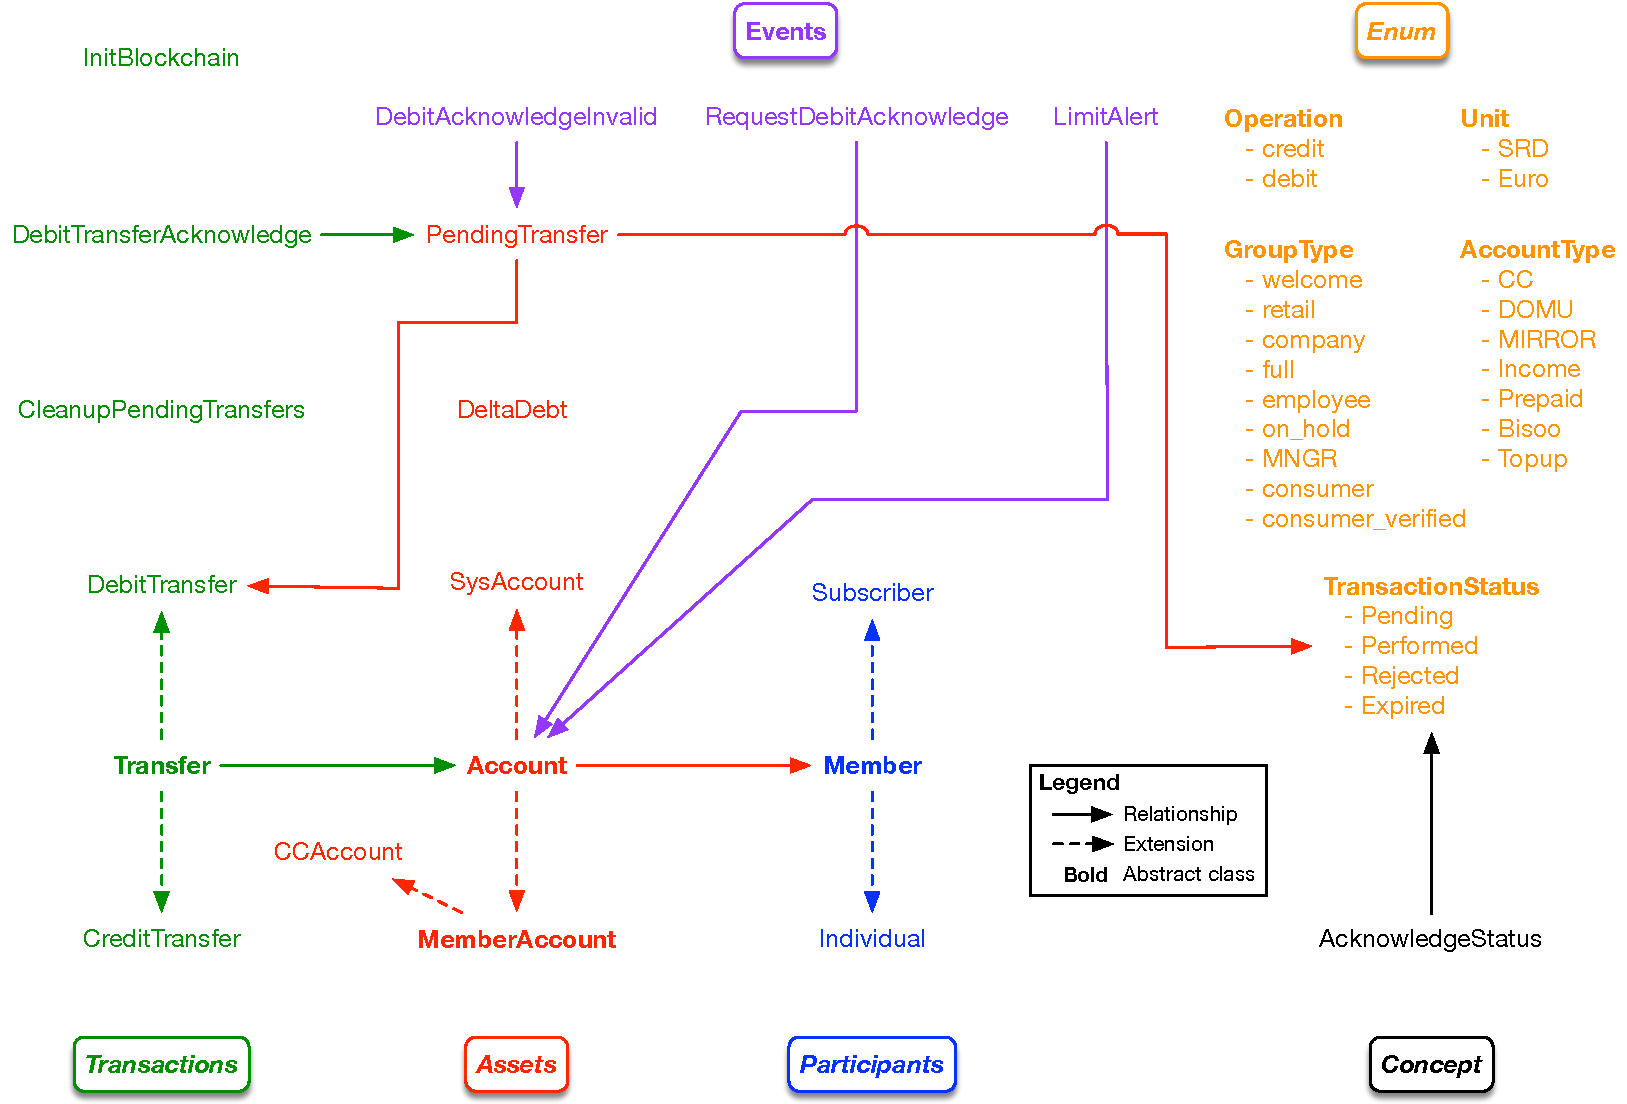
\includegraphics[width=1.0\textwidth]{Figures/cto-model}
  \caption{\bf\small CTO Model Structure used by hyperledger composer}
  \label{fig:prototype-net}
\end{figure}

In order to perform credit or debit operations a \textit{participant} need to be registered. For the prototype they are quite reduced like the assets, however, there two participants derived from \textit{Member} called \textit{Subscriber} and \textit{Individual}. Those members may own an account asset which can be used then to transfer money from one account to another one.

On several occasions event are emitted which may be consumed by an application or a user to react to specific issues happened during a transaction. There are many different events interesting for a user but for the moment there are three implemented. One is for a forecast of a possible limit violation named \textit{LimitViolation}, \textit{RequestDebitAcknowledge} asks a user to give an acknowledgement to a pending transaction and last \textit{DebitAcknowledgeInvalid} informs that the acknowledgement for a pending transaction got denied or has been invalid.

Finally there are couple of \textit{enum} types giving states names like for operations and units as well as account and group types.

A detailed explanation of the model language can be found the official hyperledger composer documentation\footnote{\url{https://hyperledger.github.io/composer/latest/reference/cto_language.html}}

\section{Prototype}
\label{sec:prototype}

The prototype is a block-chain realisation of INTERLACE, can be found on GitHub\footnote{\url{https://github.com/InterlaceProject/InterlaceBlockchain}} and is based on the specifications created in deliverable D3.1\cite{INTERLACE_D31} as well as the ASIM Specification of the requirements.

First it is necessary to install the pre-requisites which are available for Linux and Mac OS. Currently these are the recommended operating systems, however, with additional effort it might be possible to run the INTERLACE blockchain on Windows directly. To support windows user a virtual machine set-up is also available.

Additionally, it is also important to set-up a development environment described at the composer GitHub repository. If development is not planned and setting up a complete environment not necessary, it would be still recommended to install and start Composer Playground. Playground enables someone to connect, alter and test the INTERLACE payment network. Nevertheless, playground is not required and might it might be possible to use composer-cli or other methods to utilized the network.

\subsection{Install}

This part of the documents talks about how to set-up and run the business network on your machine. However, before it is actually possible to begin it is necessary to install the pre-requisites which are listed at the hyperledger composer documentation\footnote{\url{https://hyperledger.github.io/composer/latest/installing/installing-prereqs.html}}. The website also offers a download where a script for installing all the requirements for a machine is provided.

Nevertheless, for windows user those script won't help because for now most of the packages are not yet prepared (as of writing) for a windows operating systems. For this user group a virtual machine has been prepared which is also installing all the necessary frameworks and software tools during provisioning. This virtual machine is controlled by vagrant\footnote{\url{https://www.vagrantup.com/}} and uses hyper-v or virtual box as hypervisor (two different branches). That VM configuration is published at GitHub\footnote{\url{https://github.com/hirsche/hyperledger}}.

\textbf{Environment Start-Up}

Once the hyperledger environment is installed, the next step is about starting the INTERLACE environment. To make communication uniform the block-chain is configured to publish all services under the host name "interlace.chain". Windows user facilitating the suggested vagrant set-up the new hostname is added to your host-file during start-up time using the vagrant-hostmanager plug-in. Thus there is no need to configure the name manually.

\textbf{Configure Hostnames}

For non-vagrant users it is important before executing for the local set-up to add a host name entry for "interlace.chain". Usually this entry will point to ip 127.0.0.1 (localhost). On a production system or if it was chosen to start the hyperledger composer services on a public interface, the IP needs to be fixed accordingly. Here is a list of hosts-file locations according to different operating systems types:

\begin{itemize}
	\item Mac OS: /private/etc/hosts
    \item Linux: /etc/hosts
    \item Windows: C:\textbackslash Windows\textbackslash System32\textbackslash drivers\textbackslash etc\textbackslash hosts
\end{itemize}

The format may vary a little but usually a new host with its hostname is defined using it's IP and the desired host name like

\begin{lstlisting}
	127.0.0.1        interlace.chain
\end{lstlisting}

Depending on the operating system it might be also necessary to update and restart the respective services (e.g. MacOS).

\textbf{Run fabric block chain (the first time)}

Now the main configurations have been done and hyperledger fabric can be started, which acts as a base for hyperledger composer. To continue the GitHub repository \footnote{\url{https://github.com/InterlaceProject/InterlaceBlockchain}} if not yet done needs to be downloaded by using the git visioning system by calling

\begin{lstlisting}[language=bash]
	git clone https://github.com/InterlaceProject/InterlaceBlockchain.git
\end{lstlisting}

In the created directory "InterlaceBlockchain" the business network implementation including a web application can be found. The next listing shows the bash script which downloads several fabric docker container and finally starts them using docker-composer \footnote{\url{https://docs.docker.com/compose/}}:

\begin{lstlisting}[language=bash]
	cd fabric
	./downloadFabric.sh # updates images - only the first time necessary
	./startFabric.sh # start up docker environment using docker-compose
\end{lstlisting}

\textbf{Initialize Interlace-Chain}

Finally, after fabric has been started the next step is to initialize the block chain with a call of

\begin{lstlisting}[language=bash]
	cd chain
	./initNetwork.sh # use hyperledger composer to create a business network and deploy it
\end{lstlisting}

\textbf{./initNetwork.sh} will copy all models and script to the network peers to make them accessible in the hyperledger blockchain. The last step in the script starts the business network.

It may be further convenient to access network using playground and test Credit- or DebitTransfer transactions. \textbf{data.json} should act as a helper to init the network by hand, but it is recommended to update the JavaScript function \textit{initBlockchain(transfer)} in \textit{./chain/lib/init.js}. That chain-code part is executed when transaction InitBlockchain is submitted. Be careful to run \textbf{InitBlockchain} only once otherwise errors or duplicate entries might happen resulting in a inconsistent chain.

\textbf{Network updates after chain-code changes}

After changes to the acl, cto, queries, the libraries or other parts of the core chain-code application the network needs to be updated. This can be achieved by executing

\begin{lstlisting}[language=bash]
	cd chain
	./updateNetwork.sh
\end{lstlisting}

This script reads the current version number of \textit{package.json} file increases it by one and creates a new bna package. When scripts are correct and the bna-package could be created it is deployed to the peers and the network updated to a new, higher network version which will utilize the new bna package.

\textbf{Shutting down}

Sometimes it is useful to throw away everything and restart from scratch. To tear down fabric and remove card left-overs execute:

\begin{lstlisting}[language=bash]
	cd fabric
	./teardownFabric.sh
	./deletePlaygroundCards.sh
\end{lstlisting}

\textbf{Start a rest server}

Once the network is running (no playground needed) it is also possible to start a HTTP-Server which allows to interact with the network over REST. The script

\begin{lstlisting}[language=bash]
	cd chain
	./startRestServer.sh
\end{lstlisting}

starts the server and allows to get an overview of the restful interface by opening

\url{http://interlace.chain:3000/explorer}

in a browser. The REST interface itself may be contacted over

\url{http://interlace.chain:3000/}

when using it together with an external application. In case host interlace.chain has not been set-up and all the services are running locally without a VM it might be also possible to use localhost instead of interlace.chain as host name. Nevertheless, it is highly recommended to use "interalce.chain" because everything has been testing using that particular host name.

\subsection{Working with the environment}

Next a closer look is taken on how the environment might be facilitated using different approaches. It is possible to connect to the chain using composer-cli, taking advantage of composer playground (the graphical interface) or use the simple web-front-end created for the project.

\textbf{Start and test network with playground}

If you've decided to install and use Composer Playground it can be started using that command

\begin{lstlisting}[language=bash]
	composer-playground
\end{lstlisting}

The standard configuration opens a browser connecting to playground at localhost with port 8080. If you've running playground in a separate virtual environment like e.g. in a docker container, it may be necessary to start the browser manually, determine the VM-/Containers-IP and fill in the address manually in the URL field.

\textbf{The Admin Cards}

Composer Playground helps by providing a basic web interface to interact with the hyperledger fabric block-chain, on which hyperledger composer is acting as an additional wrapper. Composer creates cards in order to connect to the block-chain. These cards can be created over the playground web interface or over the command line interface. For Interlace those cards are created by \textit{initNetwork.sh} explained in section \ref{sec:prototype}. When those scripts have been executed and no error messages occurred two cards should have been created and visible when opening hyperledger playground. This is illustrated in figure \ref{fig:admin-cards}.

\begin{figure}[htbp]
  \centering
  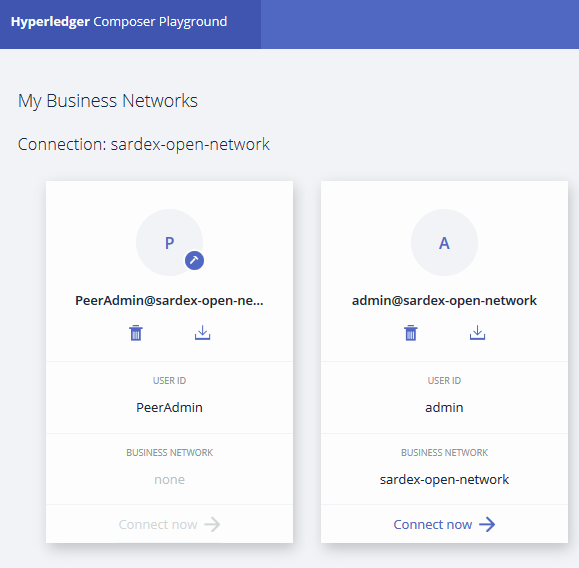
\includegraphics[width=0.5\textwidth]{Figures/admin-cards}
  \caption{\bf\small Admin Cards in Hyperledger Playground}
  \label{fig:admin-cards}
\end{figure}

Those cards provide all information needed to connect to the Interlace block-chain business network. In particular there have been installed two cards:

\begin{itemize}
	\item Peer Admin Card (PeerAdmin@sardex-open-network)
	\item Business Network Card (admin@sardex-open-network)
\end{itemize}

\textit{Peer Admin Cards} are cards (as the name suggests) used to interact with the peers. Users connecting over that card receive the permissions to manage chain-code deployments or changes on the peers. Thus it is a crucial part of every network.

Access to Interlace/Sardex Business Network is granted to another user through the provision of a \textit{Business Network Card} which is called \textit{admin@sardex-open-network}.

For Interlace we currently only have one user in place which is the admin user. However, if the network gets deployed it'll be necessary to grant acceess to other users which can be done by creating an additional Business Network Card for that particular user. Be aware that for that user a participant need to be registered first in order to link it with a new network card.

\textbf{Edit Network}

Figure \ref{fig:edit-network} illustrates how a particular business network may be edited over playground directly. For Interlace this means that you can e.g. quickly try out some changes on the JavaScript files and see if the changes are deployable by pressing the "Deploy changes"-button. However, for most developers it might prefer the usage of a common IDE\footnote{\url{https://en.wikipedia.org/wiki/Integrated_development_environment}}, which offers far better assistance during development, and use the provided scripts \textit{initNetwork.sh} as well as \textit{updateNetwork.sh}.

\begin{figure}[htbp]
  \centering
  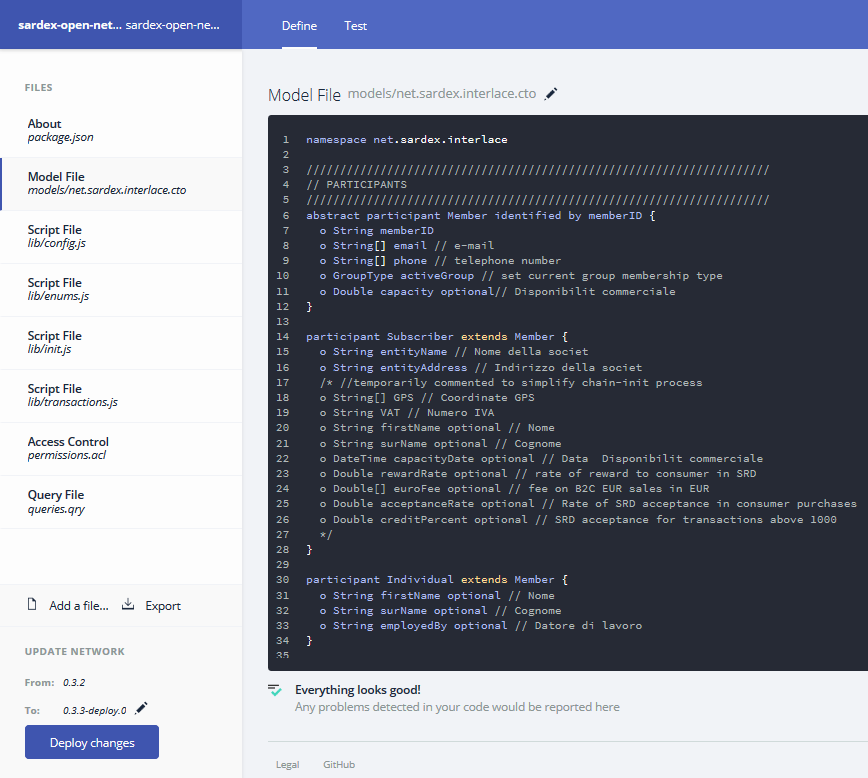
\includegraphics[width=0.6\textwidth]{Figures/edit-network}
  \caption{\bf\small Edit a network in Hyperledger Playground}
  \label{fig:edit-network}
\end{figure}

\textbf{Test Network}

The Interlace bloc-chain might be also tested directly with playground web interface instead of using the composer cli tools or launching the provided additional web application. In figure \ref{fig:test-network} you can see the playground test environment that comes with playground and is started by pressing "Test" in the menu-bar.

On the left bar of that view you are provided with a list of the Interlace participants, assets as well as entry call "All Transactions". As the menu names might suggest when clicking on them you are receiving a list of those items which have been created on the chain. E.g. this view in \ref{fig:test-network} lists all \textit{Individuals} taking part in the Interlace-Test network. When looking into the main area of the screen-shot two "Individual"-participants have been registered. One member with ID "m1" and one with ID "m2".

In addition it is possible here to add and change entries for participants and assets you might change for your customized tests.

Finally the "All Transactions" menu entry guides to a list of all transactions executed on the Interlace chain. This list contains of course not just the transactions somebody has been submitted but also entries like e.g. "AddParticipant" or "IssueIdentity", thus, all changes to the block-chain recorded can be found here.

\begin{figure}[htbp]
  \centering
  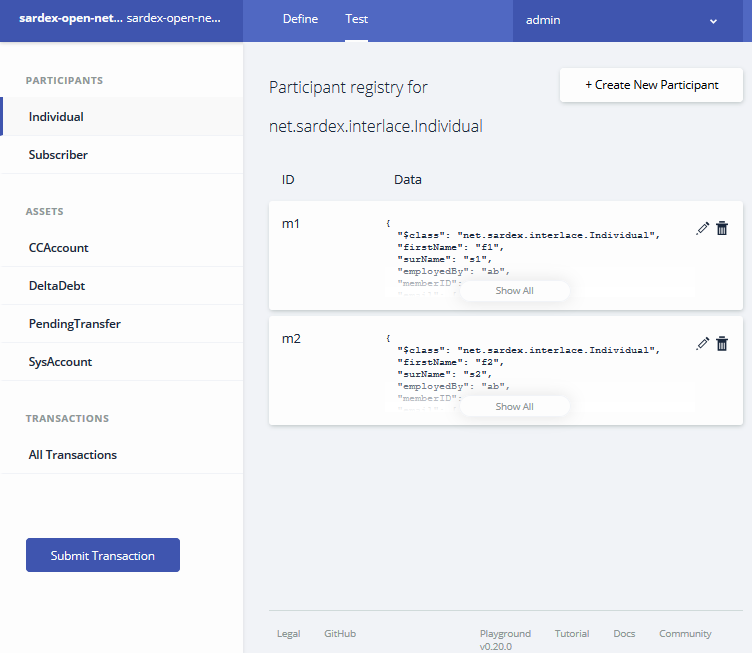
\includegraphics[width=0.7\textwidth]{Figures/test-network}
  \caption{\bf\small Test a network in Hyperledger Playground}
  \label{fig:test-network}
\end{figure}

\textbf{Submit a transaction}

In figure \ref{fig:submit-credit-transfer} a submission dialogue is shown which raises when the "Submit Transaction"-button in screen-shot \ref{fig:test-network} is pressed. This dialogue gives the possibility to select one of all possible transactions executable on the Interlace network. In this dialogue a \textit{CreditTransfer} has been selected.

In the black text-box the properties of that transactions can be provided over a JSON-String. The interface provides you with default values for the transaction specific ones.

\begin{figure}[htbp]
  \centering
  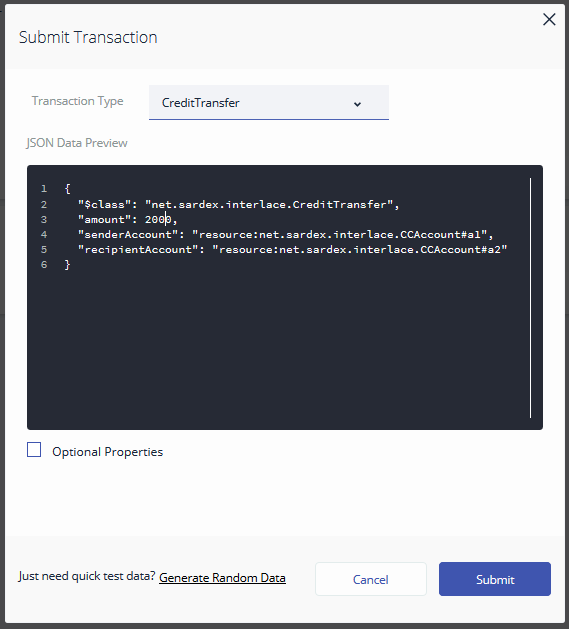
\includegraphics[width=0.5\textwidth]{Figures/submit-credit-transfer}
  \caption{\bf\small Submit a (credit) transfer in Hyperledger Playground}
  \label{fig:submit-credit-transfer}
\end{figure}

When all the necessary properties have been provided pressing "Submit" tries to commit the transaction to the block-chain. In case of an error it is shown with red text attached to the same dialogue. When everything goes as planned the transaction is endorsed, ordered and committed to peers. The resulting actions will be visible with the assets/participants as well as in the transaction log of the chain.

Details on how to configure and initialize Interlace transactions are covered in the technical details section \ref{sec:technical-details}.

\textbf{Run Transactions with composer-cli}

Init network transaction:

\begin{lstlisting}[language=bash]
	composer transaction submit -c admin@sardex-open-network -d  '{ "$class": "net.sardex.interlace.InitBlockchain" }'
\end{lstlisting}

The InitBlockchain transaction is setting up some basic accounts as well as demo members to continue with simple transactions right away.

Submit a credit transfer from account a1 to a2 with amount of 800 SRD:

\begin{lstlisting}[language=bash]
	composer transaction submit -c admin@sardex-open-network -d  '{ "$class": "net.sardex.interlace.CreditTransfer", "amount": 800, "senderAccount": "resource:net.sardex.interlace.CCAccount#a1", "recipientAccount": "resource:net.sardex.interlace.CCAccount#a2" }'
\end{lstlisting}

Submit a debit transfer from account a1 to a2 with amount of 200 SRD:

\begin{lstlisting}[language=bash]
	composer transaction submit -c admin@sardex-open-network -d  '{ "$class": "net.sardex.interlace.DebitTransfer", "amount": 200, "senderAccount": "resource:net.sardex.interlace.CCAccount#a1", "recipientAccount": "resource:net.sardex.interlace.CCAccount#a2" }'
\end{lstlisting}

A successful debit transfer creates a PendingTransfer entry with status Pending containing an OTP (one time pad). This OTP can be used by the debitor to confirm the transaction. Thus in the next example "995317396" is used to call a transaction DebitTransferAcknowledge to acknowledge the debit transfer:

\begin{lstlisting}[language=bash]
	composer transaction submit -c admin@sardex-open-network -d  '{ "$class": "net.sardex.interlace.DebitTransferAcknowledge", "transfer": "resource:net.sardex.interlace.PendingTransfer#995317396" }'
\end{lstlisting}

\textbf{The web front-end}

The web front-end currently is a simple web site generated by a yeoman generator provided by the composer-community. The web application can be found in the webapp directory.

In order to get the web application to run properly it is necessary to start-up the whole network and start the REST-server as described in the previous steps.

The web app which is based on AngularJS needs various node.js packages downloaded and installed which is achieved by calling

\begin{lstlisting}[language=bash]
	cd webapp
	npm install
\end{lstlisting}

After that a development server can be started by calling

\begin{lstlisting}[language=bash]
	cd webapp
	npm start
\end{lstlisting}

npm will start a web server at port 4200. If you work locally it also tries to open a browser which is showing the web application, otherwise you'd need start a browser manually and enter the URL by yourself. This is the URL where the server can be reached:

\url{http://interlace.chain:4200}

The web page is based on AngularJS and communicates over REST with our previously started REST server facilitating asynchronous AJAX-request.

\section{The Chain-Code}
\label{sec:chain-code}

The following part is describing the core business logic which is found in the \textit{chain} directory. The shell scripts ending with \textit{.sh} have been handled in section \ref{sec:prototype} except from \textit{startRestServer.sh} which is handled in the technical details \ref{sec:technical-details}. Given that this section focuses on the chain-code implementation which lays in the directory \textit{lib} illustrated in figure \ref{fig:chain-structure}.

\begin{figure}[htbp]
\centering
\begin{minipage}{5cm}
\dirtree{%
.1 chain.
	.2 \textbf{lib/}.
		.3 config.js.
		.3 enums.js.
		.3 init.js.
		.3 transactions.js.
	.2 \textbf{models/}.
	.2 \textbf{network/}.
	.2 connection.json.
	.2 data.json.
	.2 \textcolor{green}{initNetwork.sh}.
	.2 package-lock.json.
	.2 package.json.
	.2 permissions.acl.
	.2 queries.qry.
	.2 \textcolor{green}{updateNetwork.sh}.
	.2 \textcolor{green}{startRestServer.sh}.
}
\end{minipage}
\caption{\bf\small Chain-Code Directory Structure}
\label{fig:chain-structure}
\end{figure}


Explaining the four JavaScript files the following can be said: \textit{config.js} contains the main configurations including things like time-outs, quick-transfer-amounts, transfer-type and account type mappings which is done in form of a JSON object.

Unfortunately, composer doesn't offer static access to enumeration constants. All enumeration values of a type need to be address by a string value. That approach is quite dangerous and gives potentially space for a lot of common errors. Interlaces tries to solve this issue by setting up an object with "freezed"\footnote{\url{https://developer.mozilla.org/en/docs/Web/JavaScript/Reference/Global_Objects/Object/freeze}} attributes.

In figure \ref{lst:enumMap} a JavaScript mapping of the cto-Model enum type \textit{Unit} in \ref{lst:enumCTO} is illustrated.

\begin{center}
\begin{minipage}{0.8\textwidth}
\small
\begin{lstlisting}[language=javascript,firstnumber=1,caption={\bf\small JavaScript enumeration mapping}, captionpos=b,label=lst:enumMap]
var Unit = Object.freeze({
  'Euro': 'Euro',
  'SRD': 'SRD'
});
\end{lstlisting}
\end{minipage}
\end{center}

Using that way of enum-mapping a proper development environment is suggesting and auto-completing the possible values of an e.g. Unit when working with it. Instead there is the possibility as mentioned to directly work with string values. But writing \textit{Unit.Euro} instead of \textit{"Euro"} ensures during development when sources linted\footnote{\url{https://en.wikipedia.org/wiki/Lint_\%28software\%29}} that the correct enumeration names have been applied.

\begin{center}
\begin{minipage}{0.8\textwidth}
\small
\begin{lstlisting}[language=cto,firstnumber=1,caption={\bf\small enum in CTO-model}, captionpos=b,label=lst:enumCTO]
enum Unit {
  o Euro
  o SRD
}
\end{lstlisting}
\end{minipage}
\end{center}

\subsection{Linking Transactions}
\label{sec:link transactions}

There are two JavaScript files which contain the available transactions of the network. It is \textit{init.js} and the second one is \textit{transactions.js}. Before going into details on what these files contain a short sample is given on how transaction of the CTO-model are mapped to a JavaScript function. Listing \ref{lst:linkTransaction} gives a short example how \textit{CreditTransfer} transaction are linked to a JavaScript function with the same name.

\begin{center}
\begin{minipage}{0.8\textwidth}
\small
\begin{lstlisting}[language=javascript,firstnumber=1,caption={\bf\small Connection of JavaScript function CreditTransfer to CTO-model transaction type}, captionpos=b,label=lst:linkTransaction]
/**
 * CreditTransfer transaction
 * @param {net.sardex.interlace.CreditTransfer} transfer
 * @transaction
 */
async function CreditTransfer(transfer) { [...] }
\end{lstlisting}
\end{minipage}
\end{center}

In this example the JavaScript name of the function is not import. It is rather the annotation with \textit{@transaction} as well as defining the parameter(s) of the function and to which type they are referring to. In detail at line 3 parameter \textit{transfer} gets linked to CTO-model type \textit{net.sardex.interlace.CreditTransfer}. In case a CreditTransfer is invoked usually using a JSON string, this string is converted to a type in JavaScript which has the same properties like \textit{net.sardex.interlace.CreditTransfer} has and provided as \textit{transfer} input parameter.

Then during execution the input parameter transfer may be used like any JavaScript object and contains all the information necessary to process that transaction request. Important for the processing in JS is that the code is deterministic and evaluates to the same result on different peers.

\subsection{Init Blockchain}

The only transaction in \textit{init.js} should be only executed once otherwise it will leave you with a inconsistent block-chain if executed at all. The reason is that this initialisation script is setting up couple of participants with an account asses each to immediately test the block-chain. Thus, after the "InitBlockchain" transaction has been executed the chain contains at least two members and two accounts in order to move money around by applying credit- and debit-operations.

Listing \ref{lst:initBlock} shows parts of the actual creation of an asset as well as a participant. It uses \textit{getFactory()} which is part of the composer API to generate new instances of various types. The factory offers a function \textit{newResource} to actually create first an "Individual" from namespace \textit{net.sardex.interlace} and afterwards a "CCAccount" residing in the same namespace. The namespace is not visible in the script of \ref{lst:initBlock} because it has been configured in config.js file and applied to the config object.

Function \textit{newResource} uses namespace, type name and identifier as parameters and gives back a JavaScript representation of "net.sardex.interlace.Individual" in case of line number three. The same principle applied to line 8 when a CCAccount is created.

To write a new resource to the ledger a registry of the type super category has to be acquired.

Given that the Individual is a participant \textit{getParticipantRegistry} function need to be called in order to write it to the chain. For any asset like the CCAccount it is necessary to call \textit{getAssetRegistry} function to receive the right registry.

\begin{center}
\begin{minipage}{0.8\textwidth}
\small
\begin{lstlisting}[language=javascript,firstnumber=1,caption={\bf\small chain-code adding a new resource in \textit{initBlockchain} function}, captionpos=b,label=lst:initBlock]
let factory = getFactory();

let m1 = factory.newResource(config.NS, 'Individual', 'm1');
m1.firstName='f1';
[...]

let a1 = factory.newResource(config.NS, 'CCAccount', 'a1');
[...]
a1.balance=1000;
a1.member=factory.newRelationship(config.NS, 'Individual', 'm1');
[...]

let partReg = await getParticipantRegistry(config.NS + '.Individual');
await partReg.addAll([m1]);

let accReg = await getAssetRegistry(config.NS + '.CCAccount');
await accReg.addAll([a1]);
\end{lstlisting}
\end{minipage}
\end{center}

Once the registries are available they can be called like in line 14 and 17 with the matching type-category to finally ask for adding a new entry to the chain. Hyperledger Composer API also has  functions for reading, removing or update included. The documentation for the AssetRegistry\footnote{\url{https://hyperledger.github.io/composer/v0.19/api/runtime-assetregistry}} and for the \textit{ParticipantRegistry}\footnote{\url{https://hyperledger.github.io/composer/v0.19/api/runtime-participantregistry}} can be found in the composer documentation.

\subsection{Main Payment Transactions}
\label{subsec:main-payment-transactions}
The current implementation comes with credit and debit transactions which are working according the specifications made in D3.1 and D3.1 besides one exception explained at the end of this subsection which is talking about moving money and asset \textit{DeltaDebt}.

\textbf{CreditTransfer chain-code}

Let's now focus on the first of the two payment transactions - the credit transfers. In listing \ref{lst:js-credittransfer} the core of JavaScript function is shown without the additional function wrappers.

Code has been written in a way that is supposed to be readable by people which may not be JavaScript experts. Nevertheless, to give a quick explanation, the keyword \textit{await}\footnote{\url{https://developer.mozilla.org/en-US/docs/Web/JavaScript/Reference/Operators/await}} which deals with asynchronous JavaScript function calls and (in simplified terms) just waits till the prefixed function completes its task. If \textit{await} would be missing an asynchronous JavaScript (like previewCheck) would be called and executed in the background and the execution of the current thread would continue immediately.

\begin{center}
\begin{minipage}{0.8\textwidth}
\small
\begin{lstlisting}[language=javascript,firstnumber=1,caption={\bf\small CreditTransfer JavaScript}, captionpos=b,label=lst:js-credittransfer]
//some basic checks
await checkAmountPlausible(transfer);

// preview check throws error in case of violation
await previewCheck(transfer);

// account limits checks throws error in case of violation
await accountLimitCheck(
  transfer.senderAccount,
  transfer.recipientAccount,
  transfer.amount);

// check account limits and emits event if violated
await checkAccountLimitsAlerts(transfer.senderAccount);

// perform the transfer
await moveMoney(transfer);
\end{lstlisting}
\end{minipage}
\end{center}

The \textit{transfer}-object used in the listing is pre-filled by the chain-code API after a CreditTransfer has been invoked. It is created from the parameters and values of the JSON-object which is part of the submitted transaction and which is following the structure of the CTO-model from type \textit{net.sardex.interlace.CreditTransfer}.

\textbf{DebitTransfer chain-code}

The second function explained is the debit operation and is a bit more complex compared to a basic credit operation and shown in listing \ref{lst:js-debittransfer}. In that listing only the important part of the function is shown. The leading part calling \textit{checkAmountPlausible}, \textit{previewCheck} and \textit{accountLimitCheck} is exactly the same like in CreditTransfer and therefore left out to increase readability.

One note for debit operations resulting from the specifications is, that the owner of the senderAccount from the debit transfer is the debitor which is also the buyer. Whereas the recipientAccount owner is regarded as the creditor which is selling something.

Continuing further with the implementation, the core of the debit operation checks if an immediate transfer is possible (amount smaller than a predefined value) or if a confirmation of the other party is necessary. In case of an immediate transfer the money is moved the same way like in CreditTransfer by calling the \textit{moveMoney} function. If the transfer amount is too big a confirmation needs to be acquired from the debitor which is in our case the owner of the senderAccount of the transfer.

\begin{center}
\begin{minipage}{0.8\textwidth}
\small
\begin{lstlisting}[language=javascript,firstnumber=1,caption={\bf\small DebitTransfer JavaScript}, captionpos=b,label=lst:js-debittransfer]
// check for immediate transfer possibility
if (transfer.amount <= config.debit.quick_transfer_amount) {
  // perform the transfer
  await moveMoney(transfer);

  // check account limits and emits event if violated
  await checkAccountLimitsAlerts(transfer.senderAccount);
} else { // requires confirmation
  // add the debit transfer to the pending queue
  let otp = await insertPendingTransfer(transfer);

  // create confirmation event RequestDebitAckReqAnswCompletion
  // which is including the OTP and the sender account (of debitor)
  [...]

  // emit the event
  emit(confirmReq);
}
\end{lstlisting}
\end{minipage}
\end{center}

This is done by emitting an \textit{RequestDebitAcknowledge} event of namespace \textit{net.sardex.interlace} defined in the CTO-model which has a property \textit{otp} (One Time Pad) and a property \textit{debitorAccount} which is of type \textit{Account}. Such a DebitTransfer, which needs to be confirm, has to be stored for later. For that purpose a new asset has been created named PendingTransfer. So for every pending transfer a entry in PendingTransfer is going to be created. After than entry has been created by function \textit{insertPendingTransfer} it returns an OTP usable for the emitted event.

\textbf{DebitTransferAcknowledge chain-code}

Each entry in PendingTransfer is identified by an OTP in a way that a transfer can be unambiguously selected by providing an OTP. Currently the OTP is generated by hashing the transaction id of the debit transfer. However, if a debitor likes to confirm a transfer which he got informed by over the emitted event he just needs to pass the OTP as property for the \textit{DebitTransferAcknowledge} transaction.

\textbf{Note:} For productive Systems that identification might include an additional key as for a large numbers of PendingTransfers the OTP generated in that way might not be unique any more.

In listing \ref{lst:js-ack} the main part of \textit{DebitTransferAcknowledge}, which is different from the other transactions, is depicted. The variable \textit{ack} in the script is transaction object provided to the function, which contains the \textit{PendingTransfer} read into variable \textit{pT}. Then it is checked whether it is still in state pending, in case it is continued. In any other case an error is throws an the transaction is discarded (!not! recorded into the ledger).

If the process is continued the timestamp of the transaction is checked against the \textit{expires} date property of the pending transfer. Consequently, if expired, the state is updated to \textit{"Expired"} and function \textit{DebitTransferAcknowledge} returns with a respective status (\textit{AcknowledgeStatus}).

\begin{center}
\begin{minipage}{0.8\textwidth}
\small
\begin{lstlisting}[language=javascript,firstnumber=1,caption={\bf\small RequestDebitAcknowledge JavaScript excerpt}, captionpos=b,label=lst:js-ack]
[..]
//get pending transaction
let pT = ack.transfer;

// varify state of pending transfer
if (pT.state !== TransactionStatus.Pending) {
  throw new Error('Transfer is not in state "' +
    TransactionStatus.Pending + '" but in state "' + pT.state + '"');
}

// varify if pending transaction has been expired
if (ack.timestamp >= pT.expires) {
  //update state from Pending to Rejected
  await updatePendingTransaction(pT, TransactionStatus.Expired);

  //prepare return message
  rS.status = TransactionStatus.Expired;
  rS.description = 'OTP ' + pT.otp + ' is expired.';
  return rS; //TODO: raise event
}
[..]
\end{lstlisting}
\end{minipage}
\end{center}

The later parts of the function after all of the checks have been passed and the debit transaction can be performed the execution steps are pretty much the same like in a CreditTransfer. The only difference is that in case of success or error the PendingTransfer asset of the transaction need to be update to Performed or Rejected respectively. A function called \textit{updatePendingTransaction} also used in line 14 of listing \ref{lst:js-ack} takes care of putting the asset PendingTransfer into the right state.

Additionally in all cases \textit{updatePendingTransaction} has been applied also a status object called \textit{AcknowledgeStatus} is created and return by the function which contains the resulting status but also an error message in case something went wrong.

\textbf{moveMoney \& DeltaDebt}

Actual movement of an amount from one to an other account is performed by basic addition/subtraction of the respective account and finally updating the account assets in the ledger by facilitating the registry offered by hyperledger composer API.

Another important step, however, which is part of that money transfer and shown in listing \ref{lst:js-movemoney} is a additional functionality and has not been explained in the former requirements documents of the Interlace project. This logic collects all debts, thus, every transactions which are causing the balance to get negative or to increase an already negative balance. Those debts are collected because they are handled similar to a loan. They don't cause any additional fees, nevertheless, those debts are having a due date till when they need to be paid back. For details of debt collection you may be also referred to the appendix.

\begin{center}
\begin{minipage}{0.8\textwidth}
\small
\begin{lstlisting}[language=javascript,firstnumber=1,caption={\bf\small moveMoney JavaScript excerpt}, captionpos=b,label=lst:js-movemoney]
[..]
// check balance if DeltaDebt entry needs to be added
// !after amount has been substracted!
if (transfer.senderAccount.balance < 0) await createDeltaDebt(transfer);
// check balance if clearing an open DeltaDebt is necessary
// !before amount has been added!
if ((transfer.recipientAccount.balance - transfer.amount) < 0) {
  await clearDebt(transfer);
}
[..]
\end{lstlisting}
\end{minipage}
\end{center}

The creation of a debt handled by \textit{createDeltaDebt} is straight forward and just adds an entry to asset \textit{DeltaDebt} if a transaction has been detected which causes a negative balance or increases an already negative balance. A new \textit{DeltaDebt} entry receives an original amount, a current amount, an owner id and of course a due date when it needs to be paid back.

If soever a transaction is adding money to the account owners balance former \textit{DeltaDebt} entries may be cleared which is done by querying all debts with an non-paid amount. This is illustrated in listing \ref{lst:js-cleardebt} where a rich query called \textit{selectDeltaDebt} is used to get all of those unpaid debts. Details that and other queries are discussed in subsection \ref{subsec:queries}.

\begin{center}
\begin{minipage}{0.8\textwidth}
\small
\begin{lstlisting}[language=javascript,firstnumber=1,caption={\bf\small clearDebt JavaScript excerpt}, captionpos=b,label=lst:js-cleardebt]
// query result sorted by "oldest" first
let openDelta =
  await query('selectDeltaDebt', {ID: (transfer.recipientAccount.member.memberID)});
\end{lstlisting}
\end{minipage}
\end{center}

All selected debts are iterated starting by the oldest first. The available portion of the amount gets subtracted from the current DeltaDebt asset. If the amount is bigger than the debt the rest of the amount is used in the next iteration step to clear the nearest (in terms of age) entry of delta debt. Thus this loop continues either till there is no amount left or all debts have been paid back which also means that the balance goes back having a positive value.

\subsection{Additional Transactions}

\todo{Cleanup Pending Transfer}

\subsection{Queries}
\label{subsec:queries}

\todo{}

\subsection{ACL-file}

\todo{}

\subsection{Deployment}

\todo{}


\section{Web Application}
\label{sec:webapp}

\todo {describe}

\section{Further Technical Details}
\label{sec:technical-details}

\todo {rest server https://hyperledger.github.io/composer/latest/reference/rest-server}